This section describes the dynamic behaviour of the system in the most relevant cases.

The following sequence diagrams highlight the runtime interactions between clients, servers and the database; in the case of internal interaction between sub-components of the Application Server, these interactions are expanded and detailed. This is not the case with the client applications, since the internal structure is simpler and there is no need to further detail said relations.

Direct interactions between the Application Server and the Database are not explicitly represented, since such interactions are abstracted by the persistence unit of the Application Server.

\begin{figure}[H]
\begin{center}
		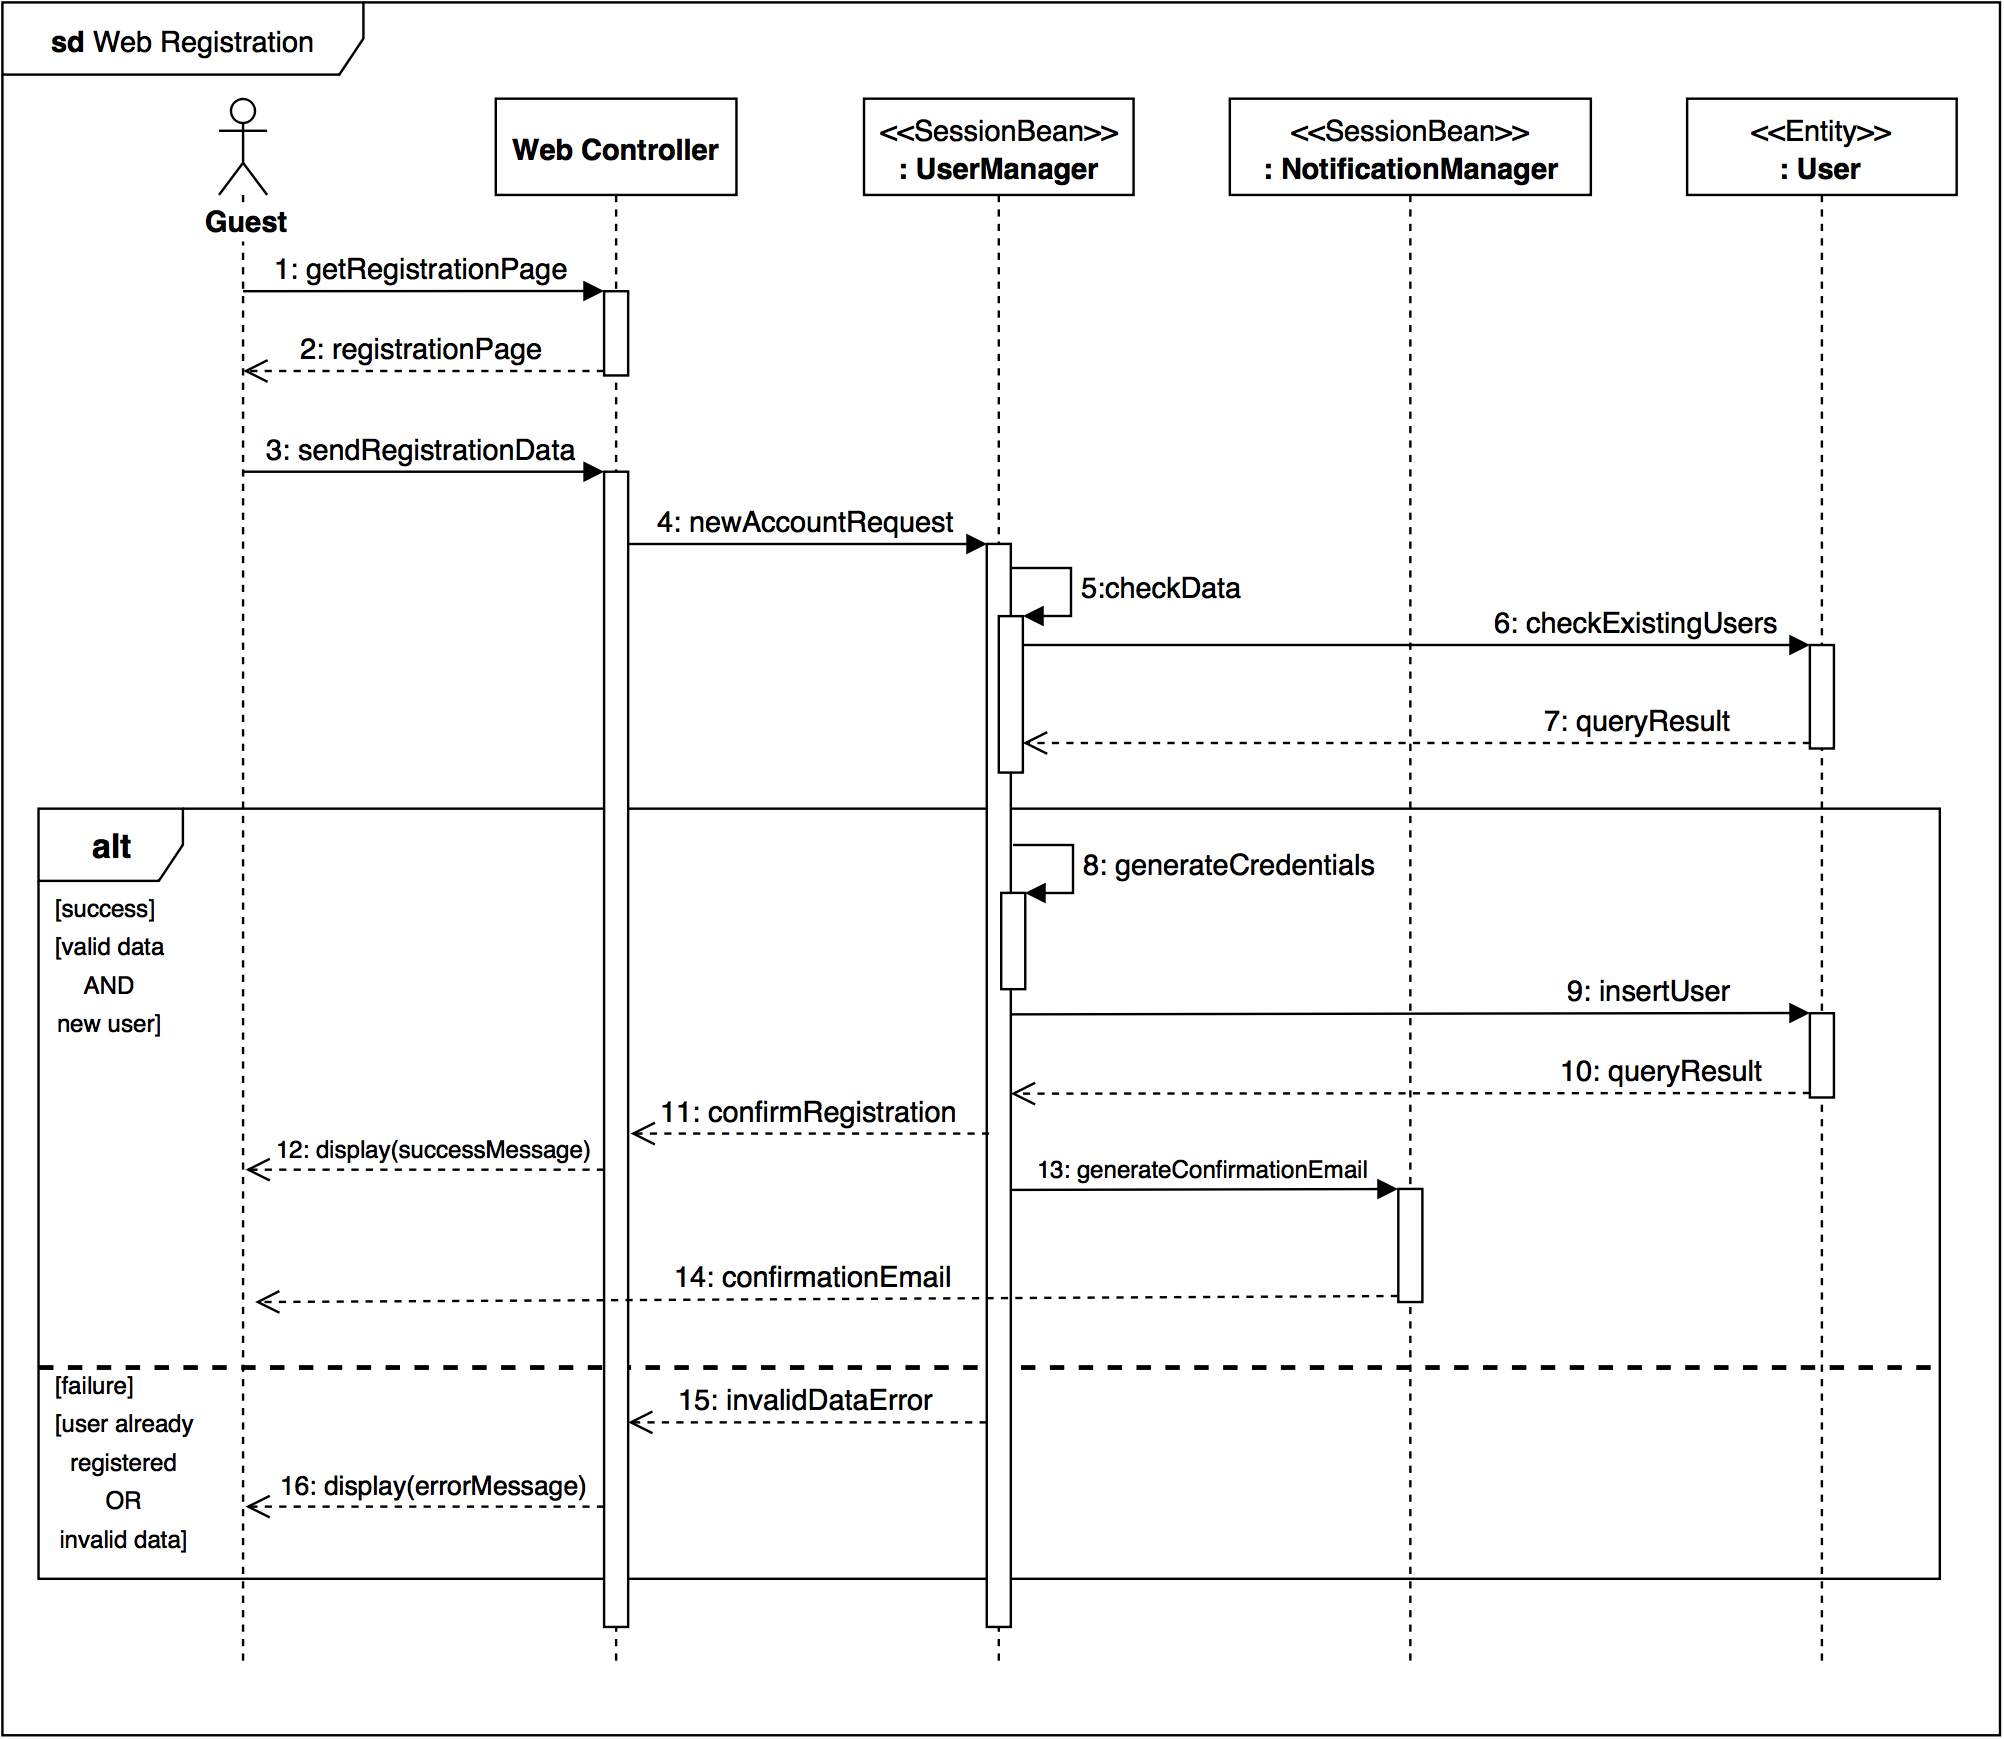
\includegraphics[width=\textwidth]{./arch_design/diagrams/registration_sd.png}
		\caption{Sequence diagram of the registration process via the web browser client.}
		\label{registration_sd}
\end{center}
\end{figure}

\begin{figure}[H]
\begin{center}
		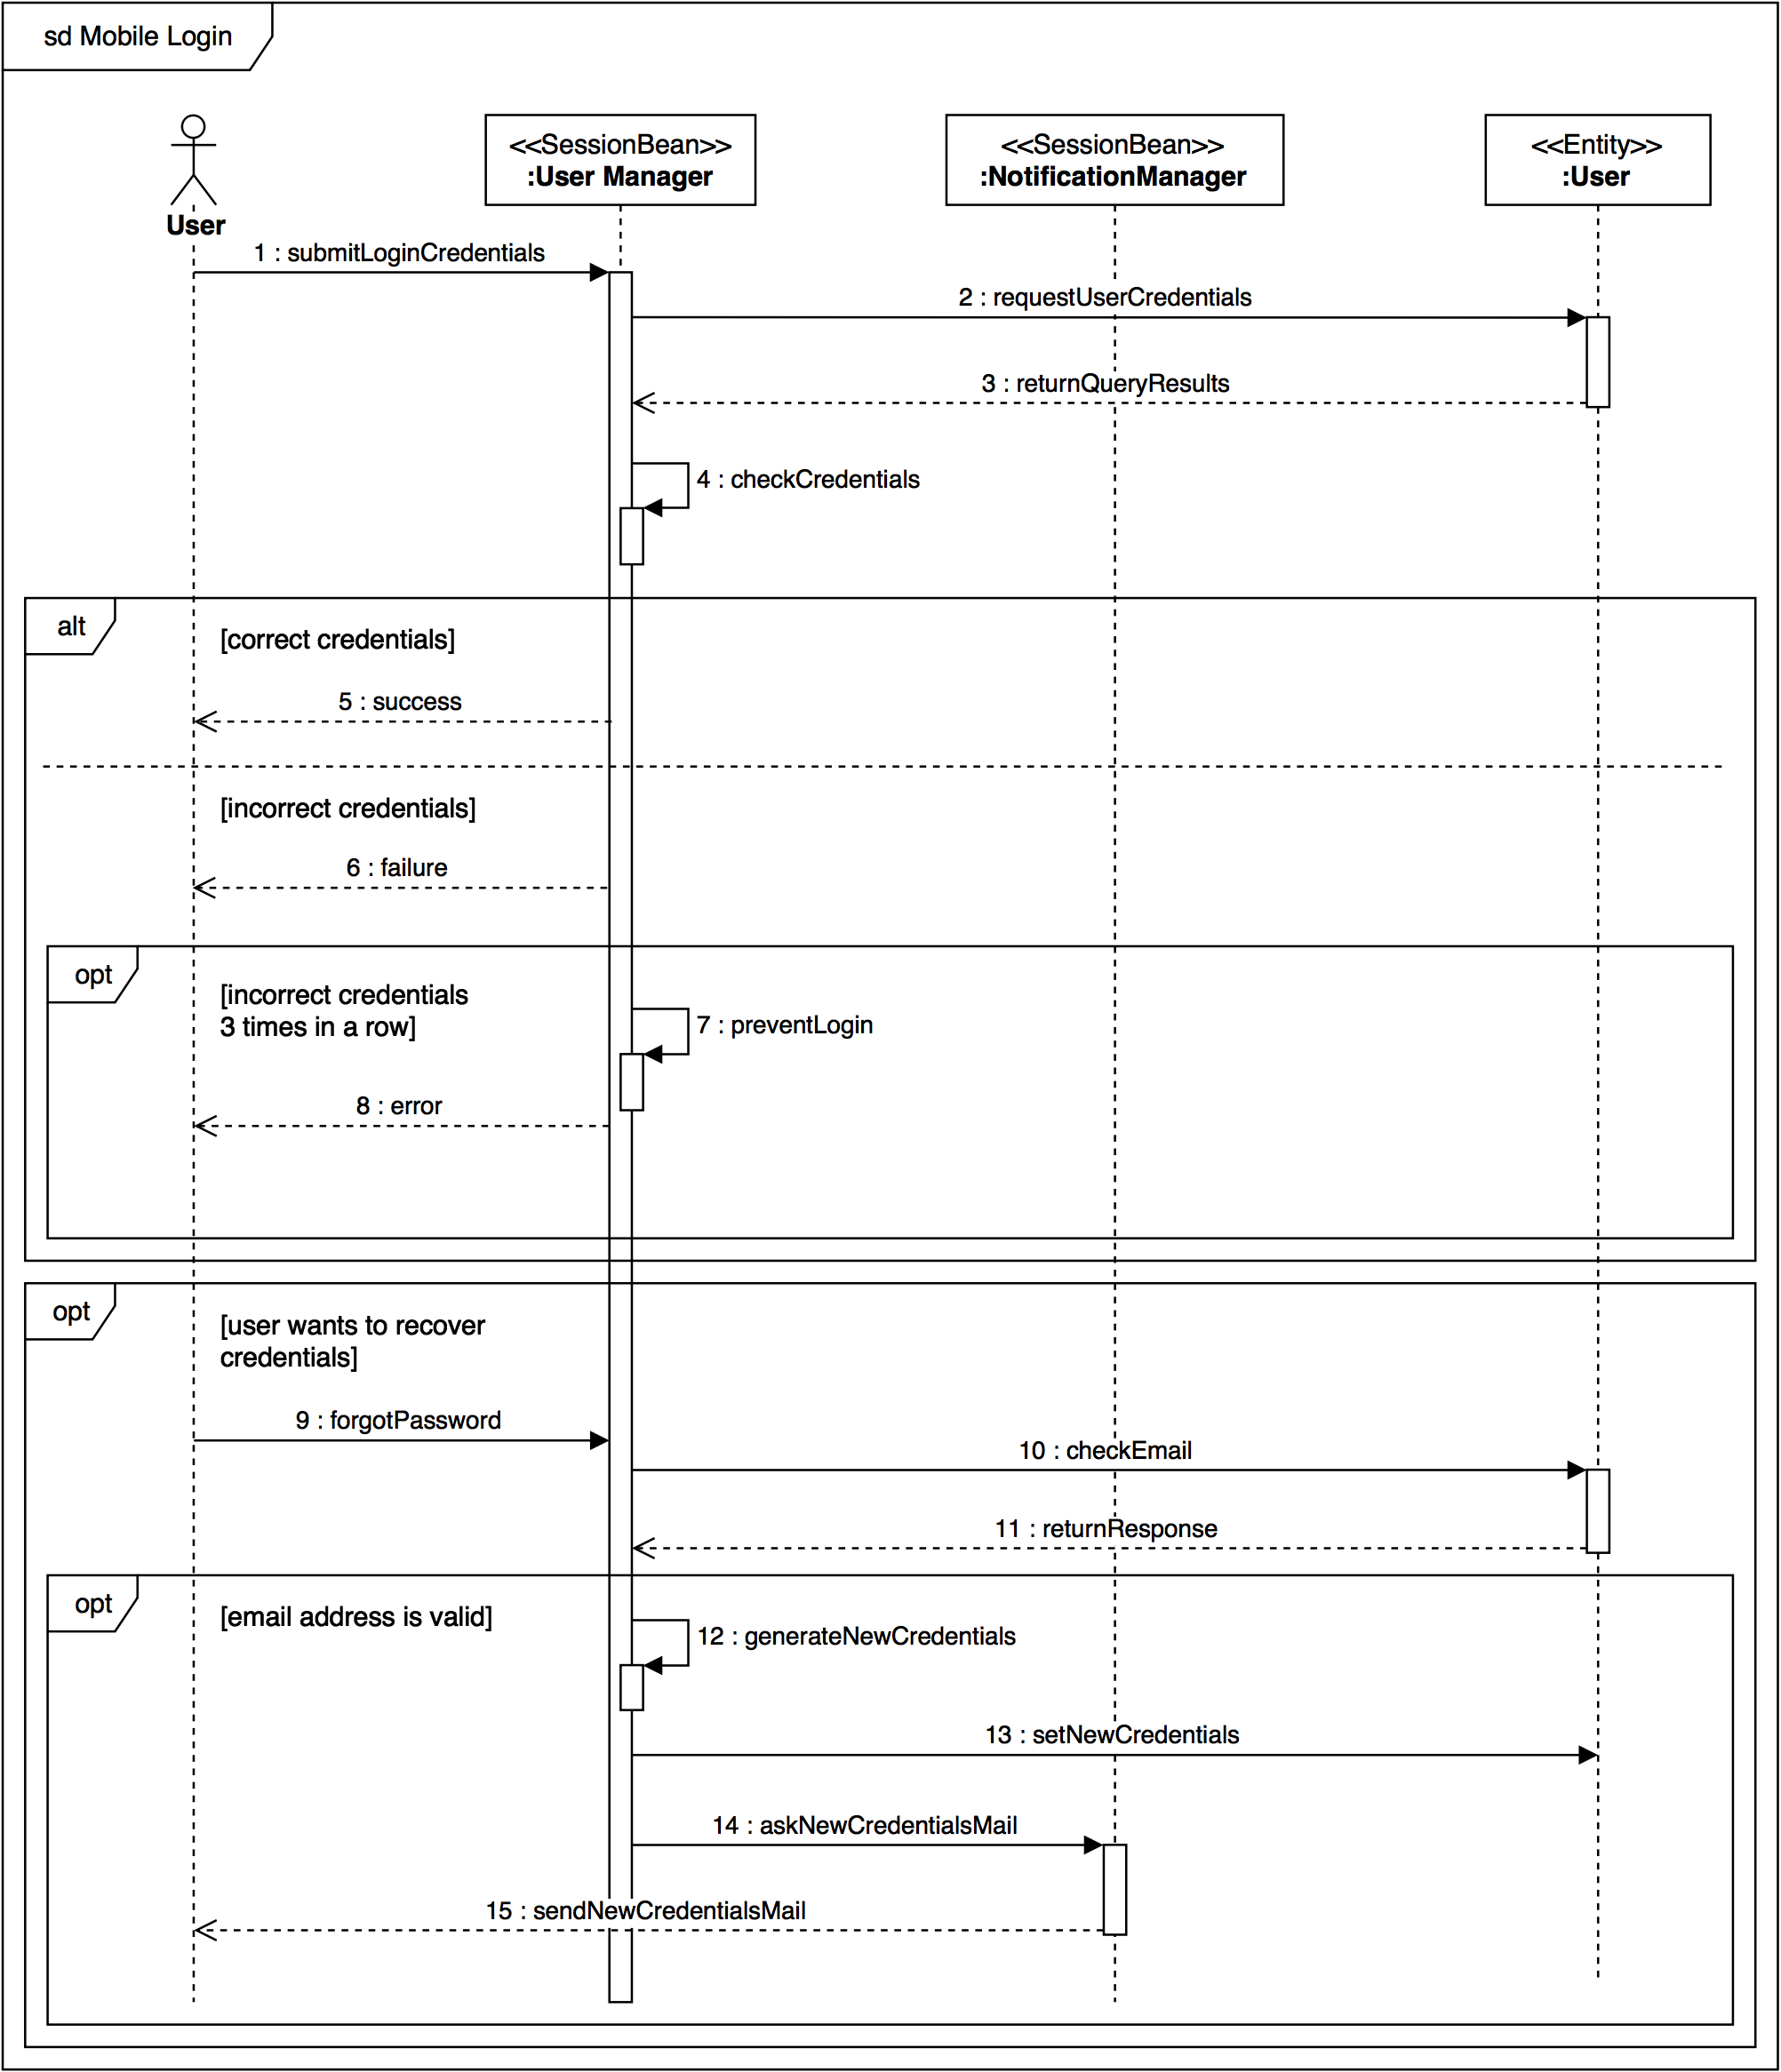
\includegraphics[width=\textwidth]{./arch_design/diagrams/login_mobile.png}
		\caption{Sequence diagram of the login process and password recovery via the mobile application client.}
		\label{login_sd}
\end{center}
\end{figure}

\begin{figure}[H]
\begin{center}
		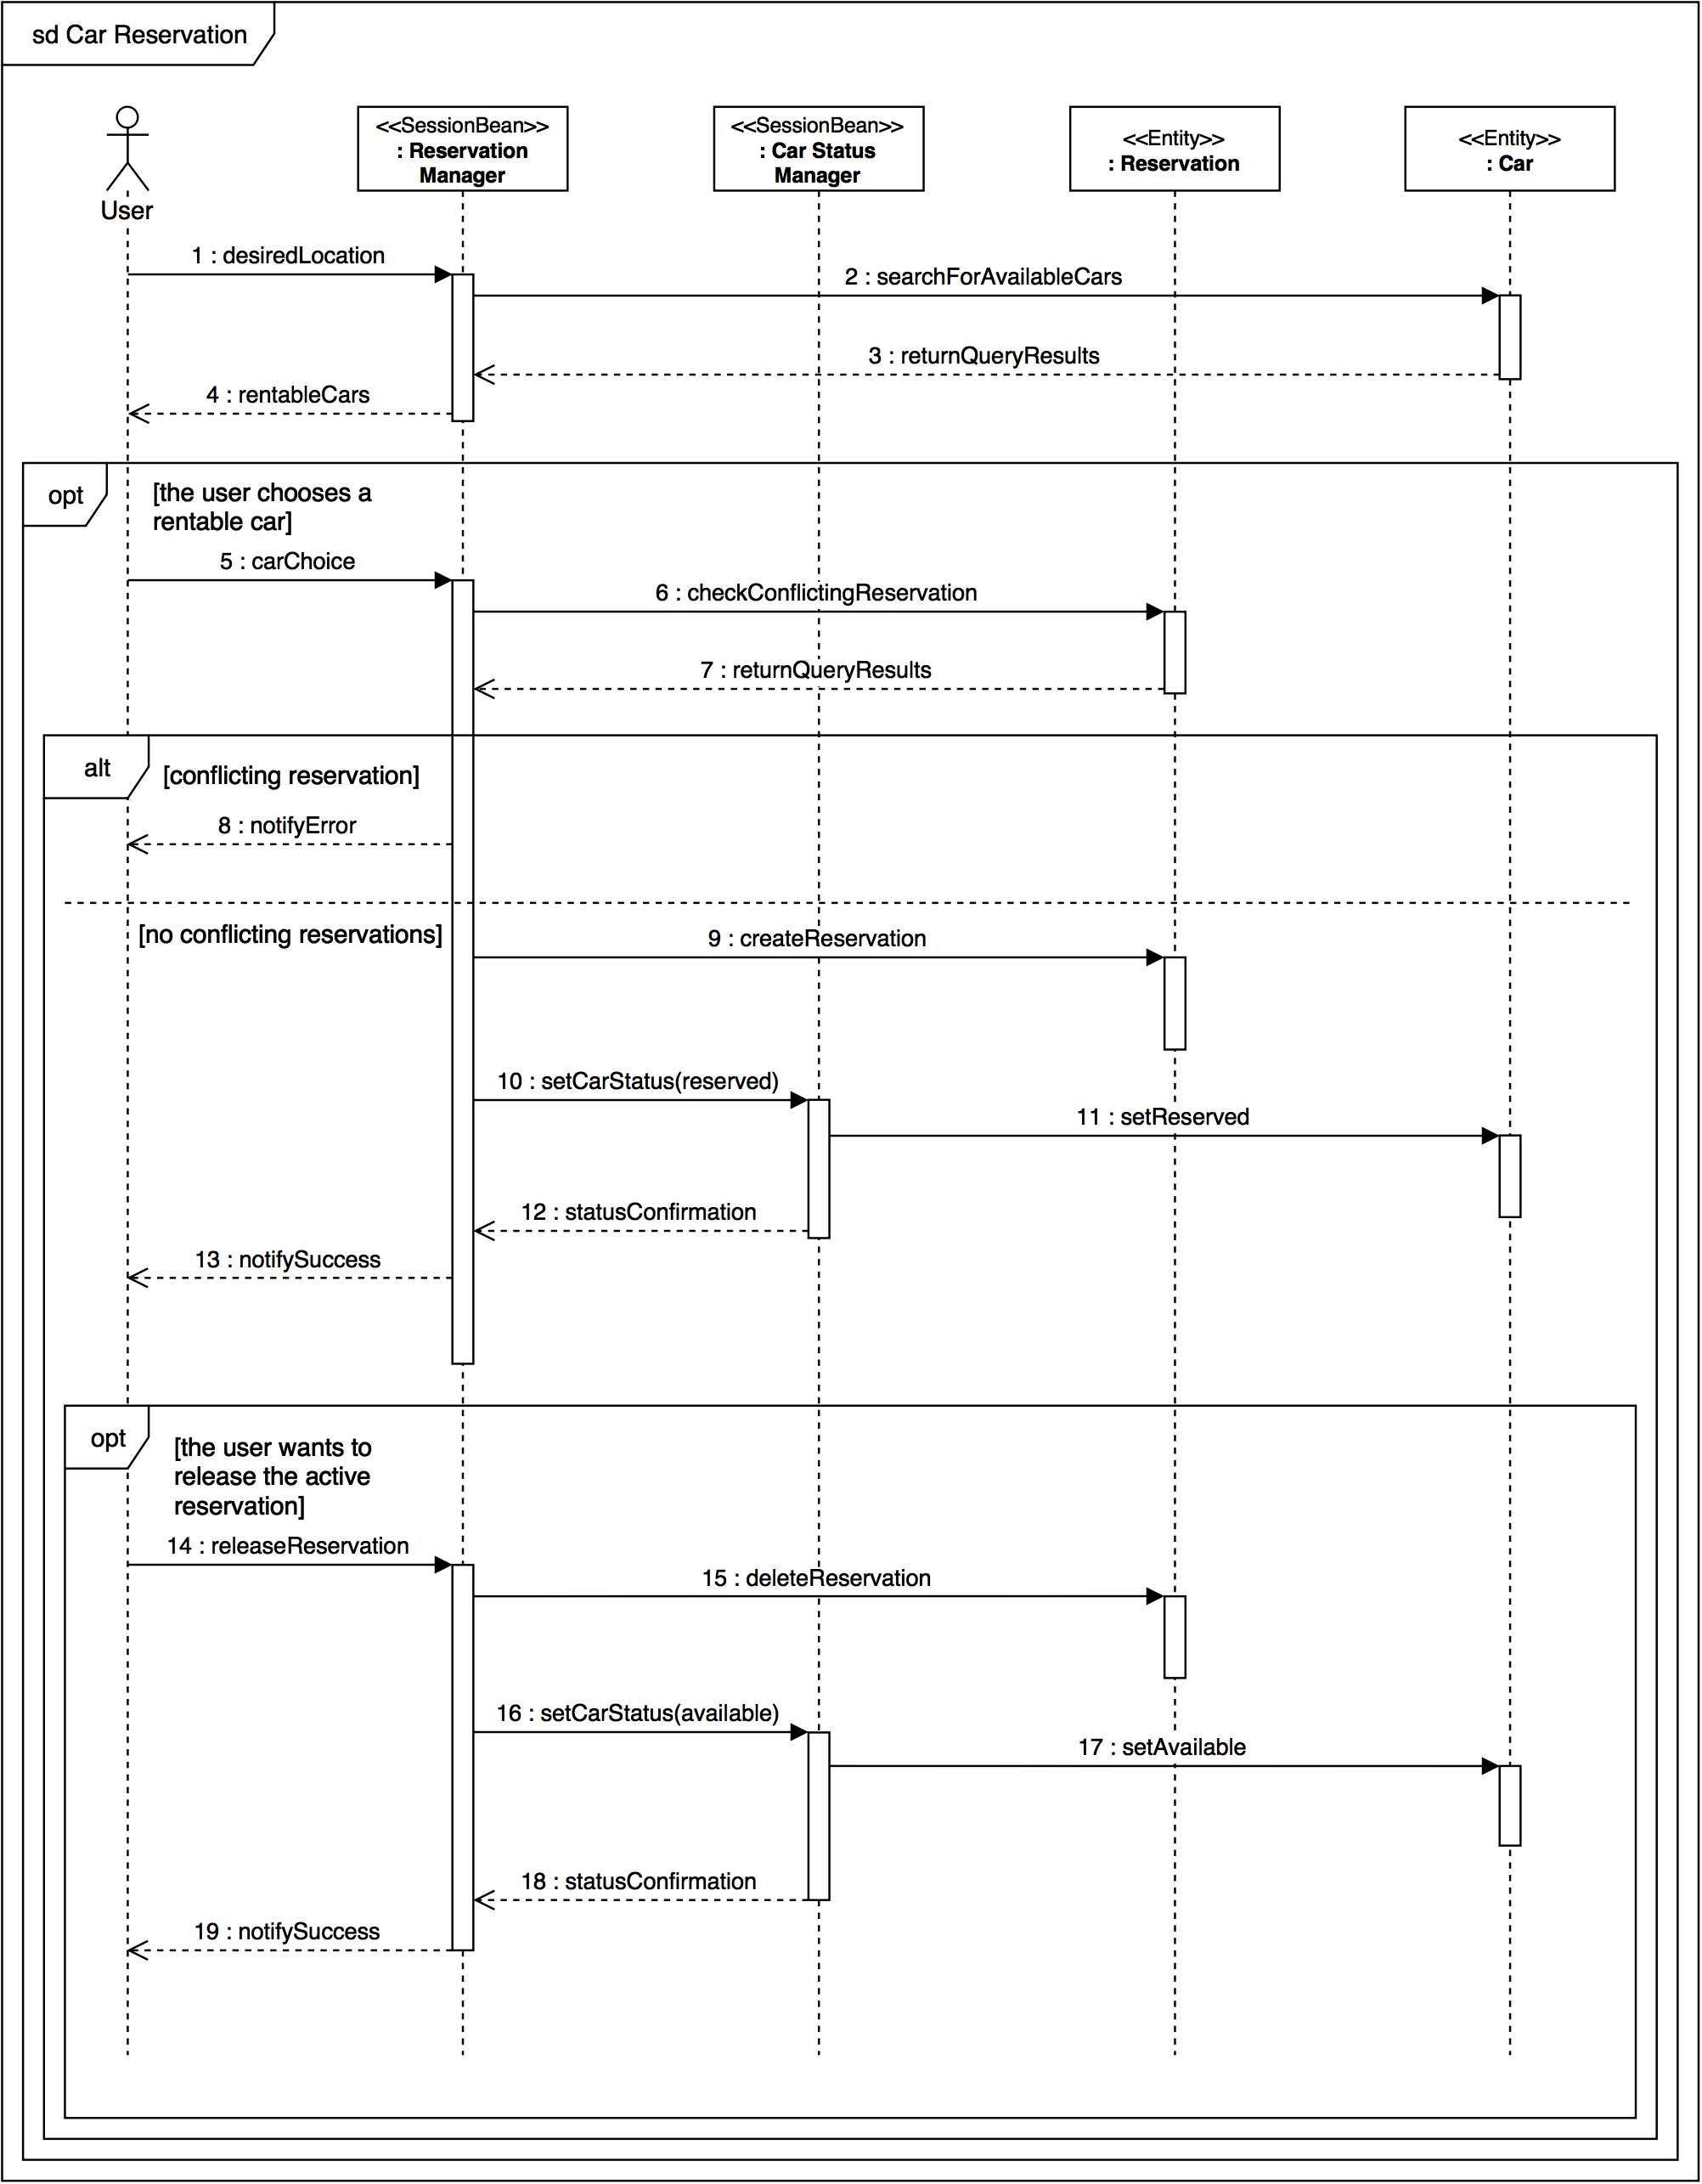
\includegraphics[width=\textwidth]{./arch_design/diagrams/car_reservation_sd.png}
		\caption{Sequence diagram of the reservation and releasing reservation processes via the mobile application client.}
		\label{reservation_sd}
\end{center}
\end{figure}

\begin{figure}[H]
\begin{center}
		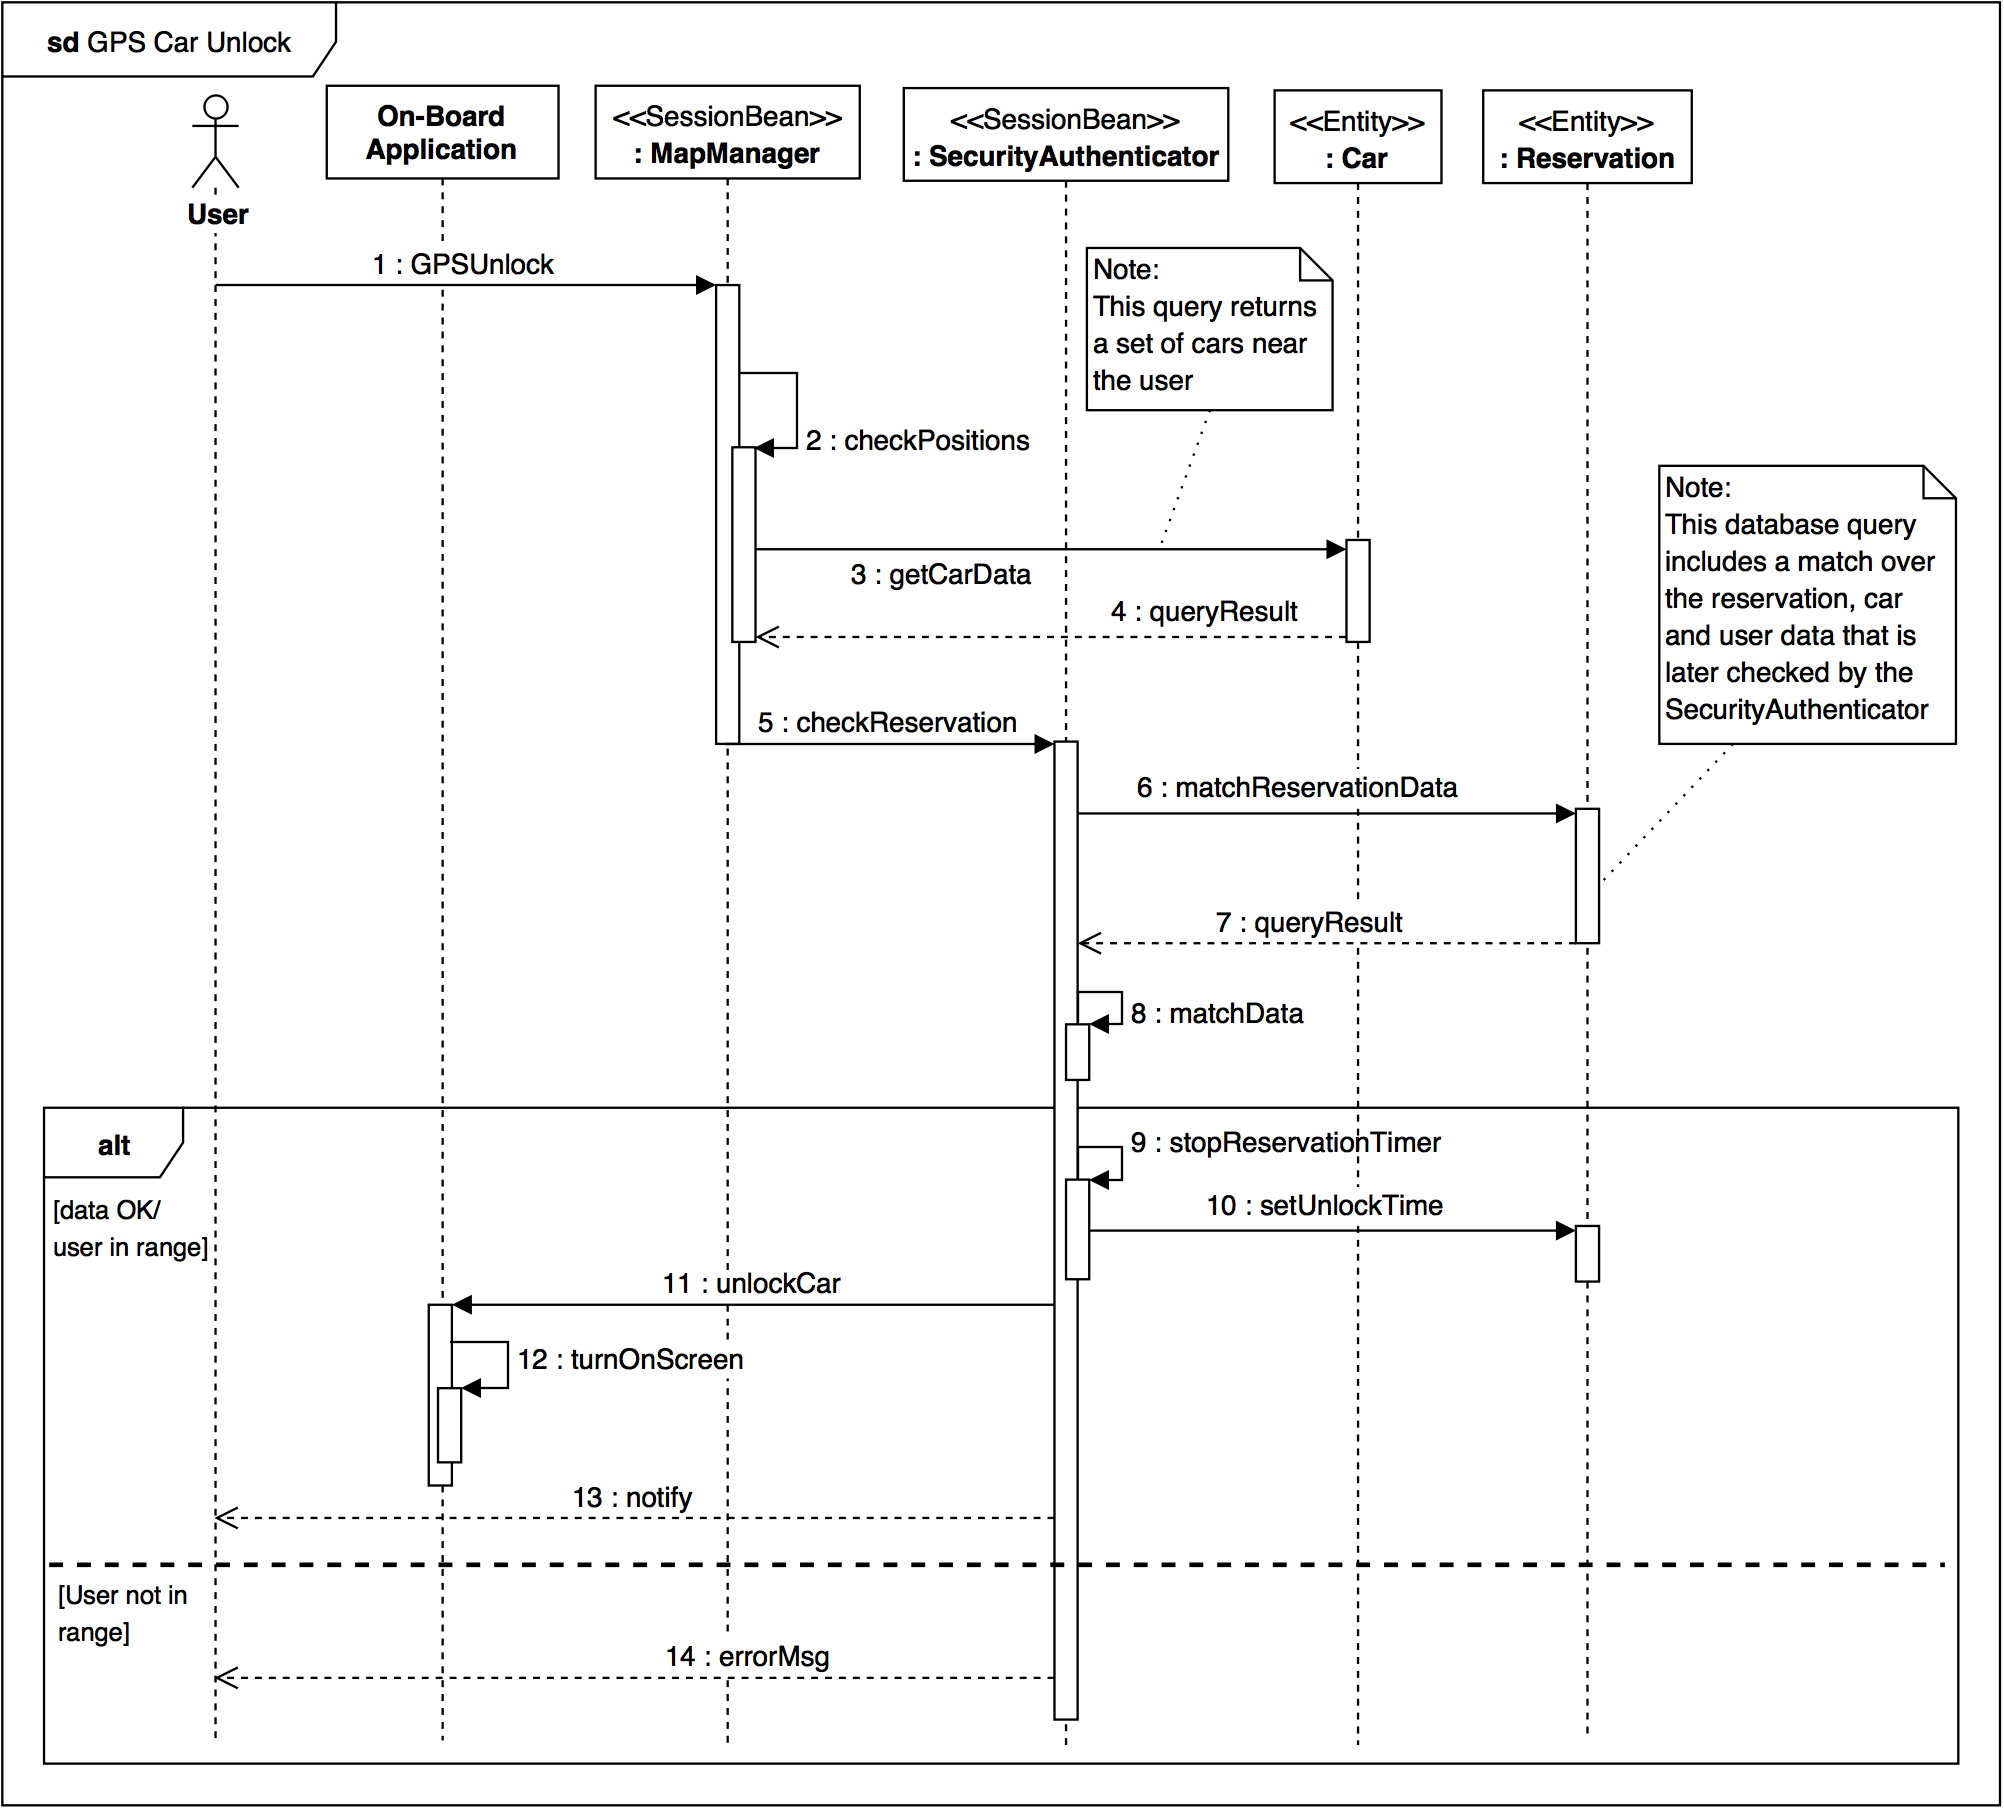
\includegraphics[width=\textwidth]{./arch_design/diagrams/gps_unlock_sd.png}
		\caption{Sequence diagram of the car unlocking process using the GPS method.}
		\label{gps_unlock_sd}
\end{center}
\end{figure}

\begin{figure}[H]
\begin{center}
		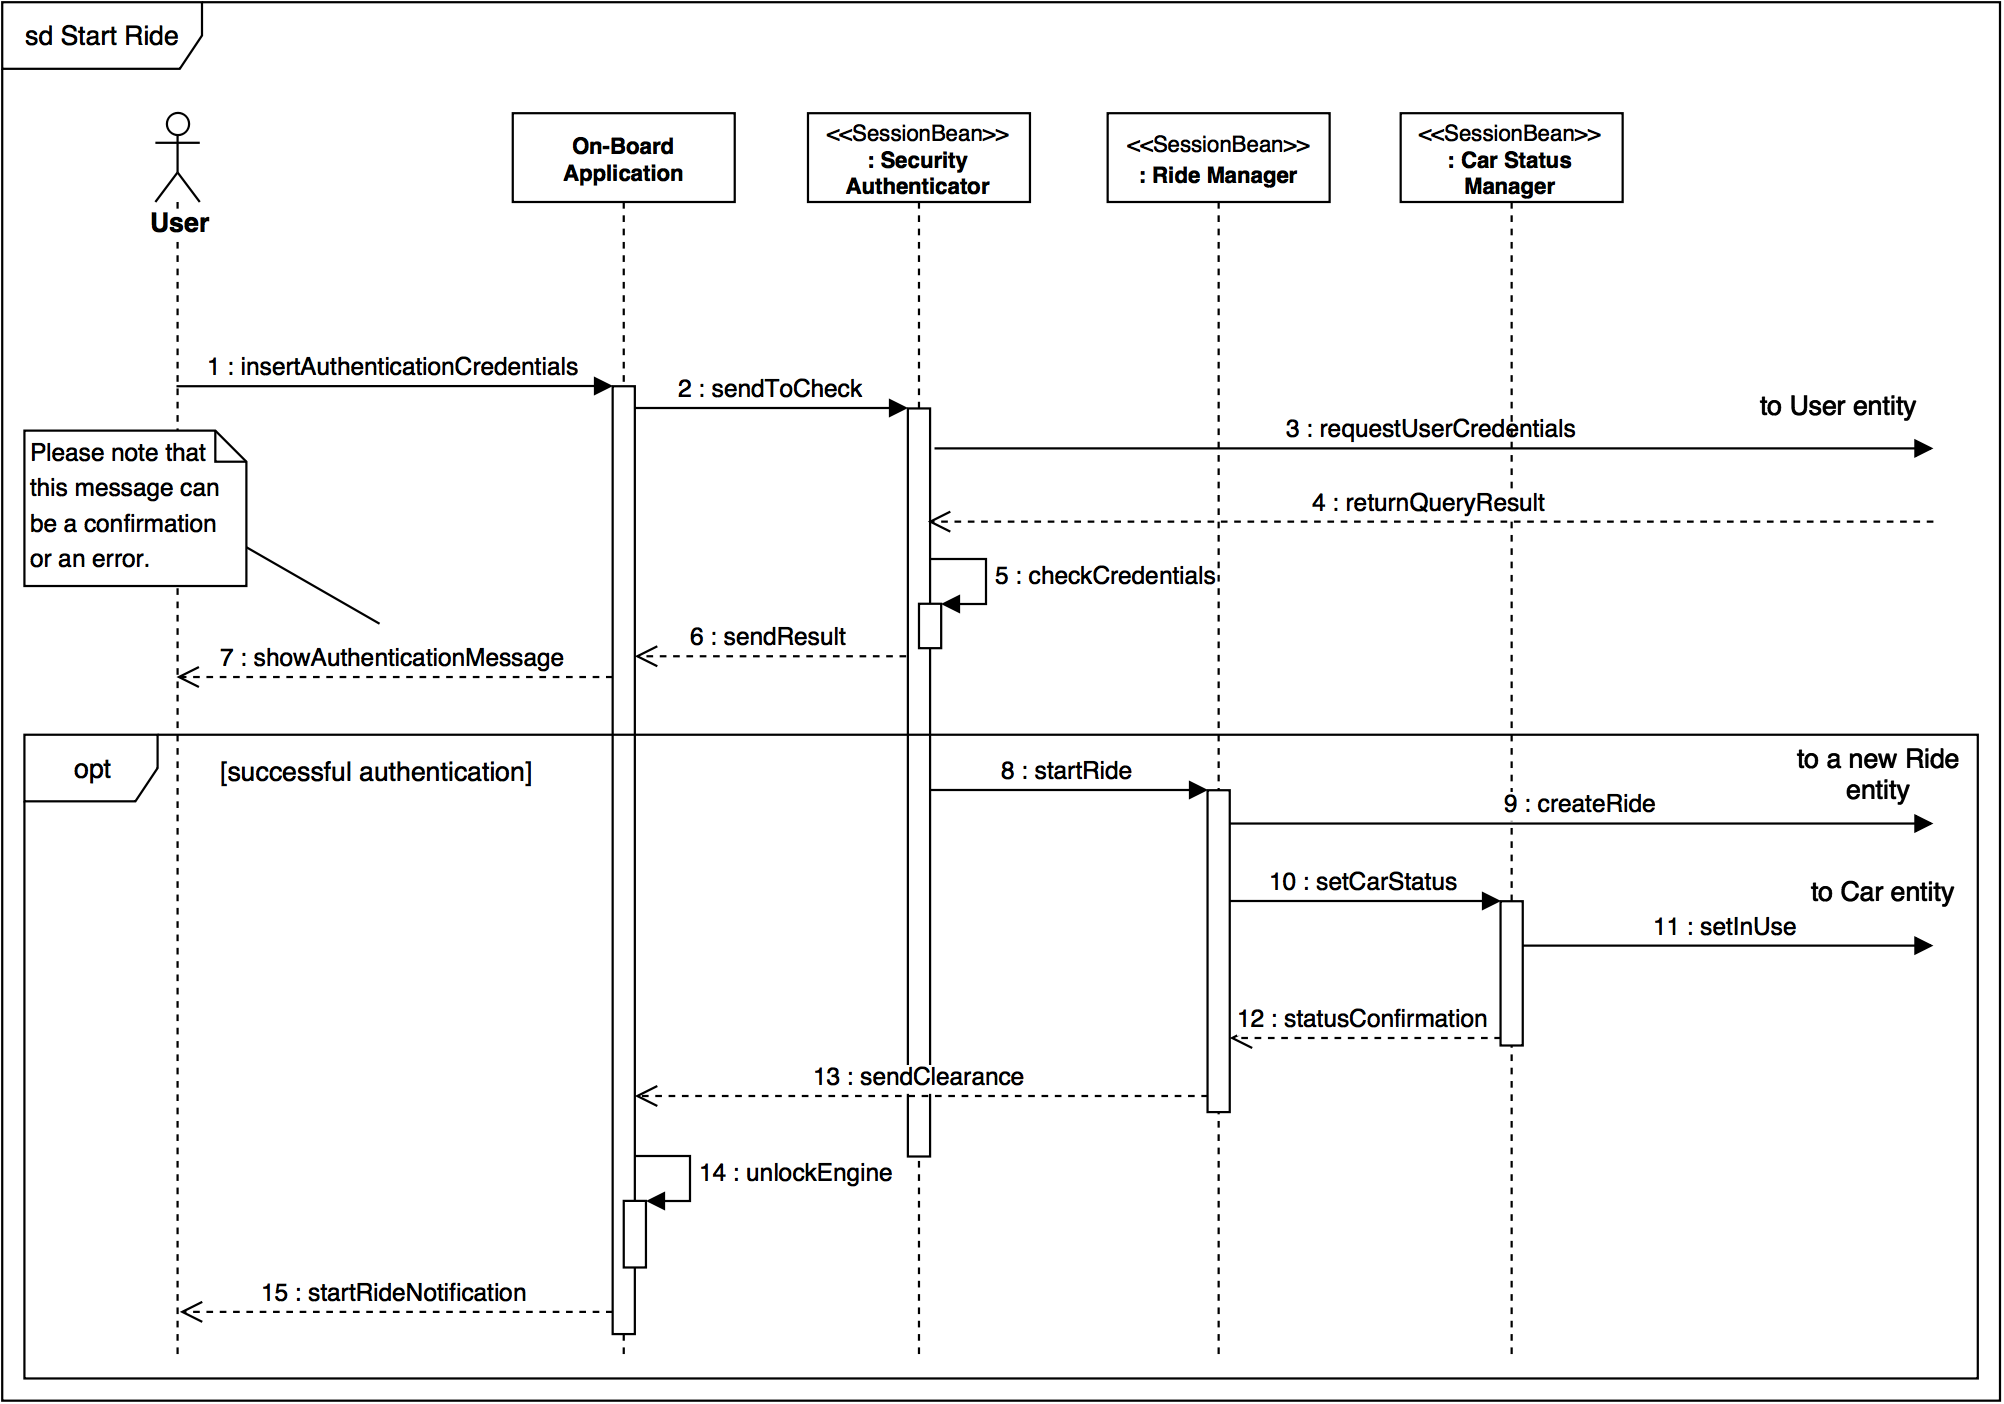
\includegraphics[width=\textwidth]{./arch_design/diagrams/start_ride_sd.png}
		\caption{Sequence diagram of the start ride process.}
		\label{start_ride_sd}
\end{center}
\end{figure}

\begin{figure}[H]
\begin{center}
		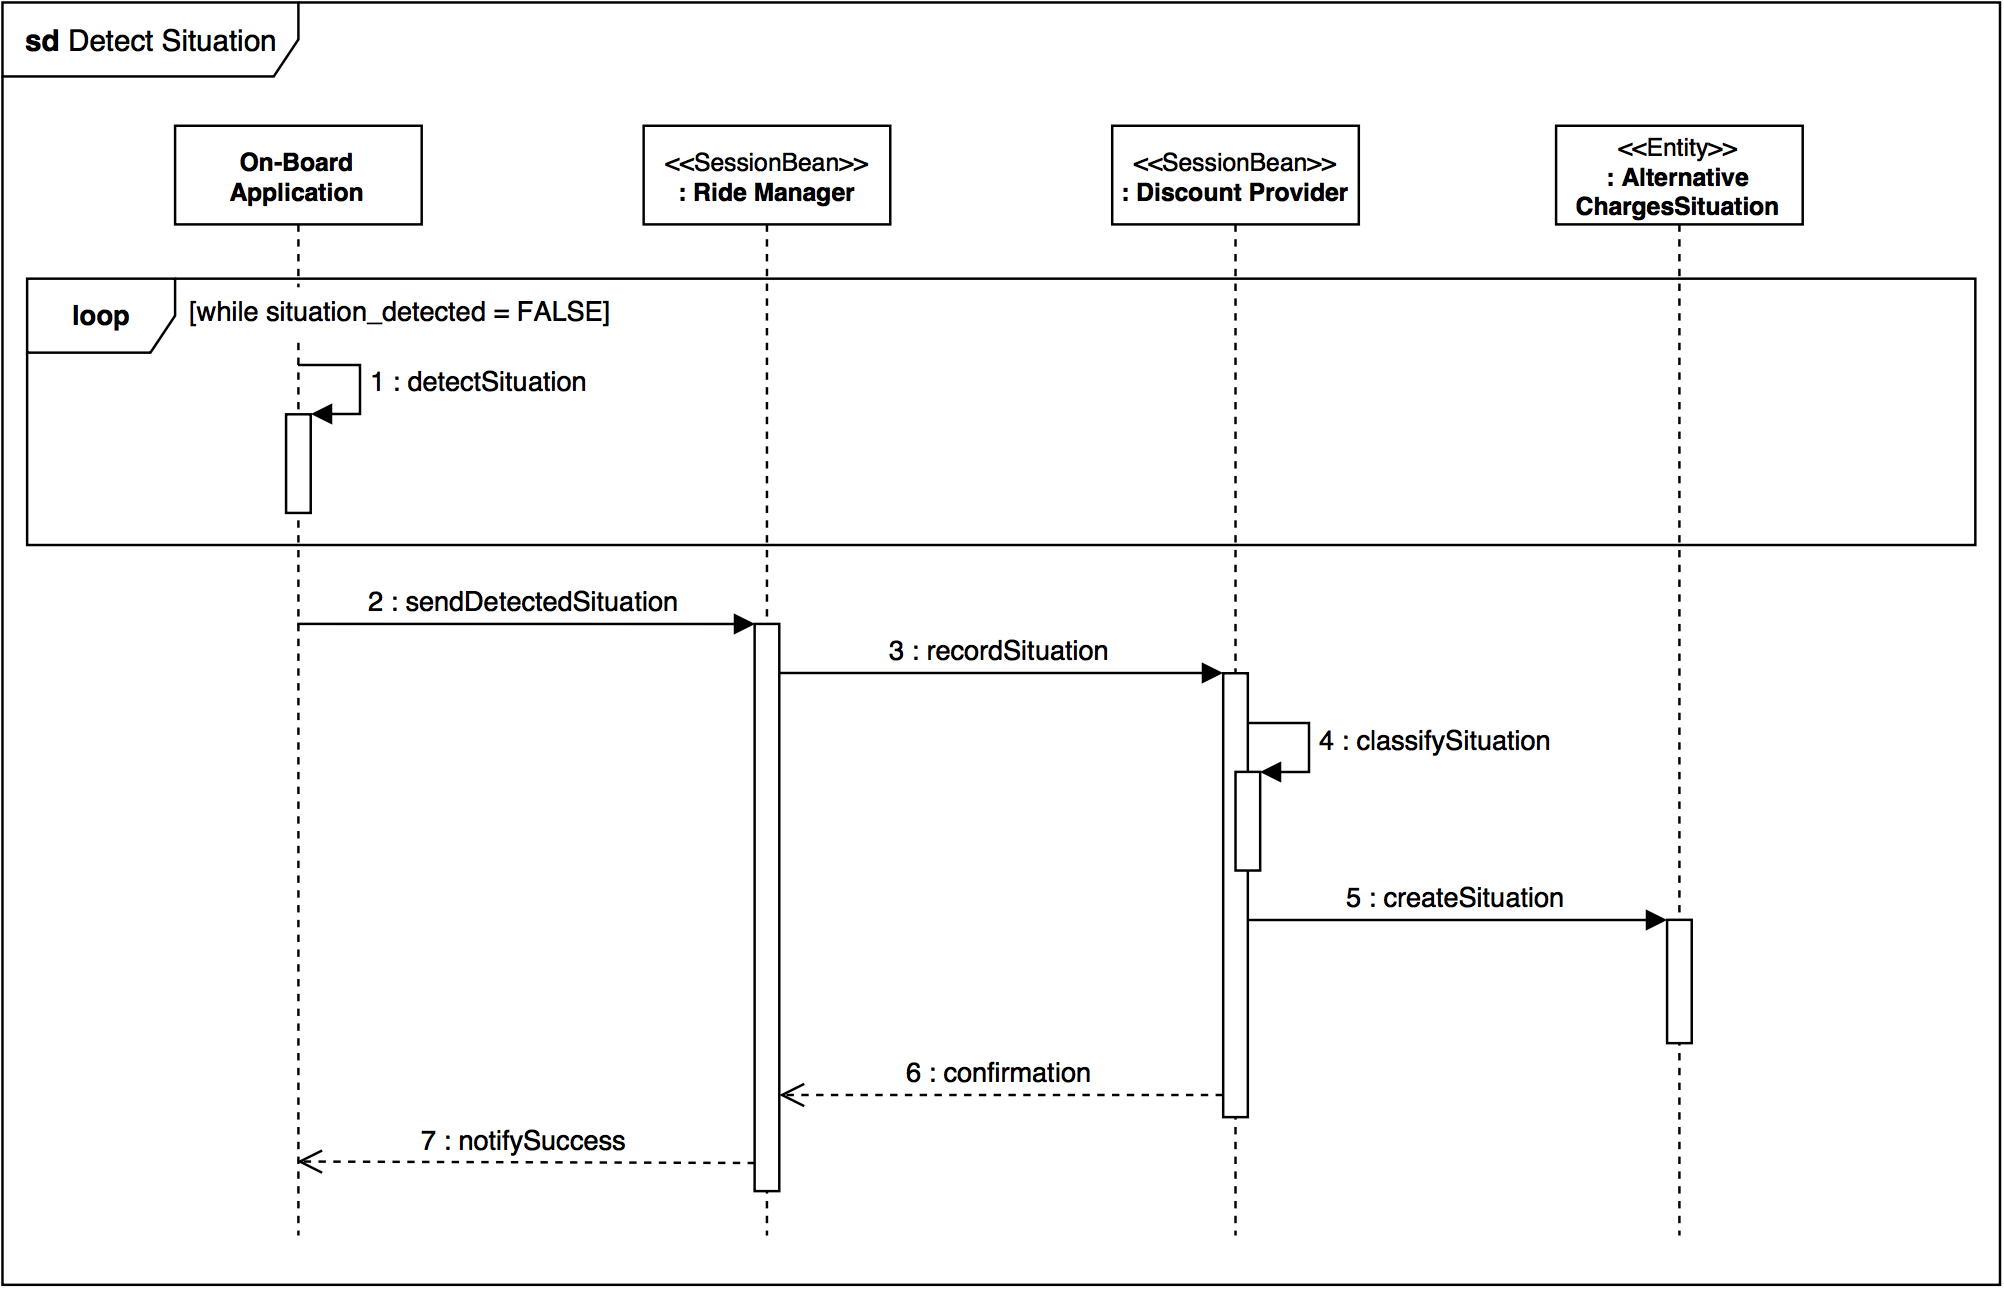
\includegraphics[width=\textwidth]{./arch_design/diagrams/apply_bonus_sd.png}
		\caption{Sequence diagram of discount/additional charges situations detection and storage processes.}
		\label{apply_bonus_sd}
\end{center}
\end{figure}
\begin{figure}[H]
\begin{center}
		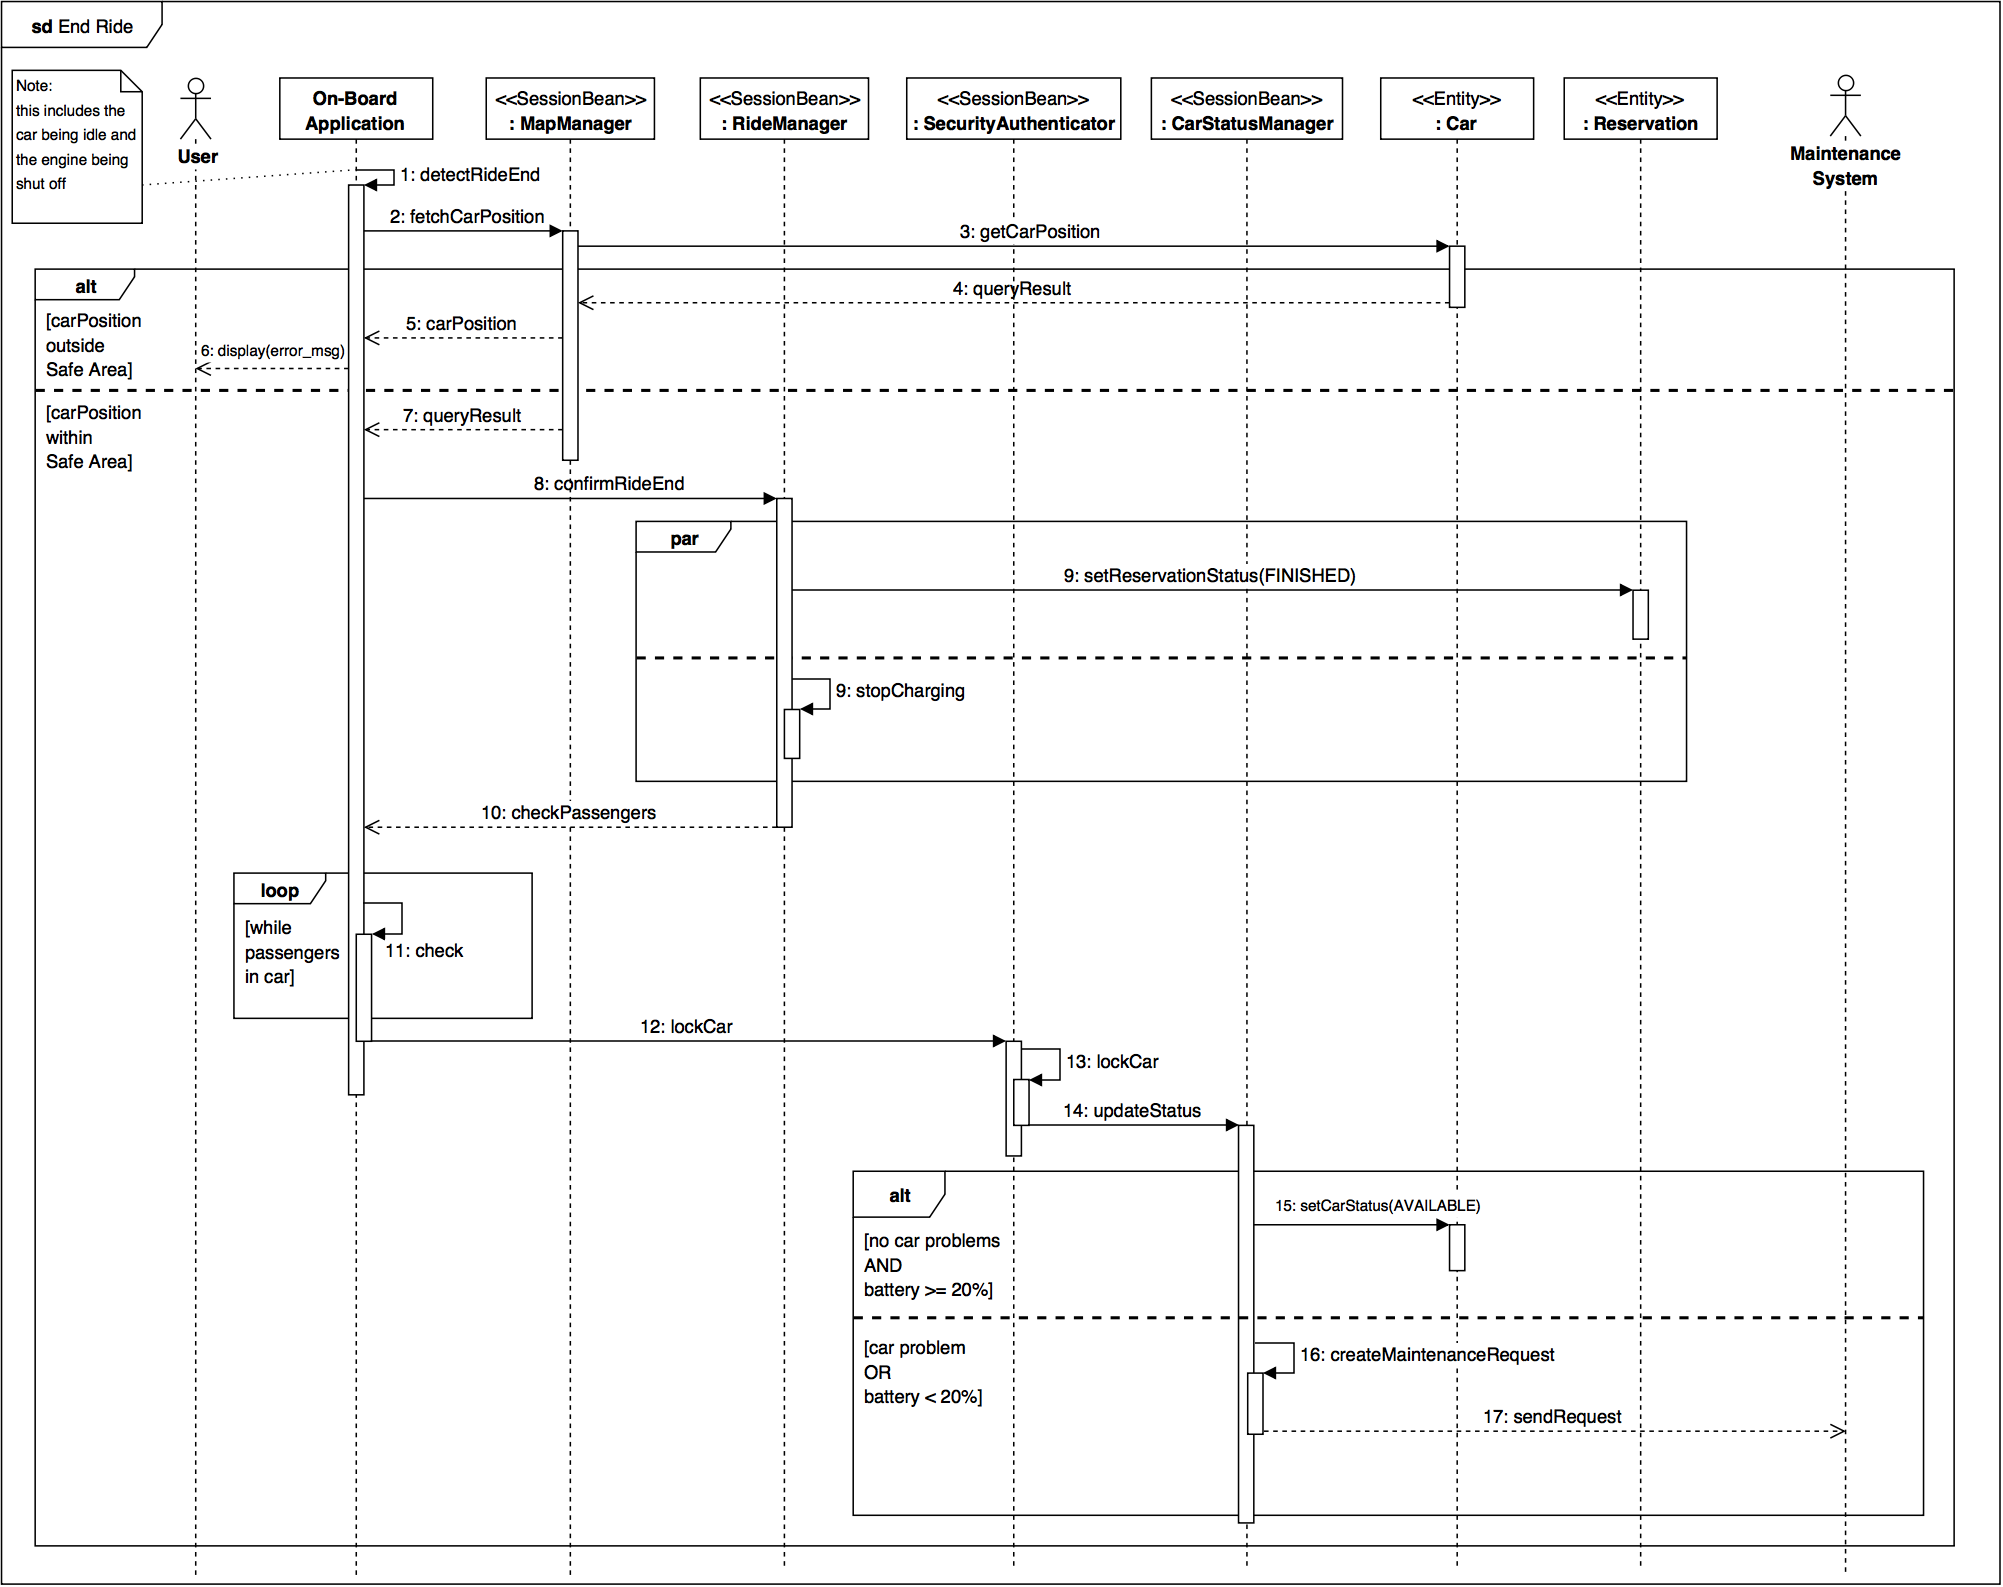
\includegraphics[width=\textwidth]{./arch_design/diagrams/end_ride_sd.png}
		\caption{Sequence diagram of the end ride process, highlighting the possibility to contact the Maintenance System in case of emergency after the end of the ride.}
		\label{end_ride_sd}
\end{center}
\end{figure}